\section{Objetivos}
 O objetivo principal desta prática é a simulação em Matlab de um sistema de controle digital completo dado as equações em Z que descrevem os blocos constituintes do sistema em malha fechada.

\section{Fundamentação Teórica}
Para realização desta prática se utilizou a teoria da transformada Z inversa, em específico o método das equações de diferenças

\textcolor{red}{DESCREVER O MÉTODO}

\section{Procedimentos}
O exercício consistiu em simular um sistema de tempo discreto para período de amostragem de 0,1 s para sinal de entrada uma onda quadrada de amplitude 0 - 5 V, com período de 10s e 2\% de ruído randômico. O sistema está mostrado na Figura \ref{fig:pr2_esquema}, bem como as equações dos blocos estão descritas abaixo:

\begin{equation}
C(z) = 0,9*\frac{z-0,8}{z-1}
\label{pr_2_C}
\end{equation}

\begin{equation}
	G(z) = \frac{0,3z}{(z-0,5)(z-0,2)}
    \label{pr_2_G}
\end{equation}

\begin{equation}
	S(z) = \frac{0,2}{z-0,8}
    \label{pr_2_S}
\end{equation}

\begin{figure}[!th]
	\centering
    \includegraphics[scale = .5]{Imagens/Execicio1_pr2.PNG}
    \caption{Diagrama de blocos da prática 2.}
    \label{fig:pr2_esquema}
\end{figure}

\section{Resultados e discussões}
\textcolor{red}{COLOCAR A DEDUÇÃO DA EQUAÇÃO DE DIFERENÇA DO PROBLEMA}

O código implementado em Matlab está mostrado abaixo:
\lstinputlisting{Arquivos_tex/Aula_5_Exercicio_2.m}

Obtendo como saída o gráfico da Figura \ref{saida_ex2_pr_2}.

\begin{landscape}
  \begin{figure}[!ht]
      \centering
      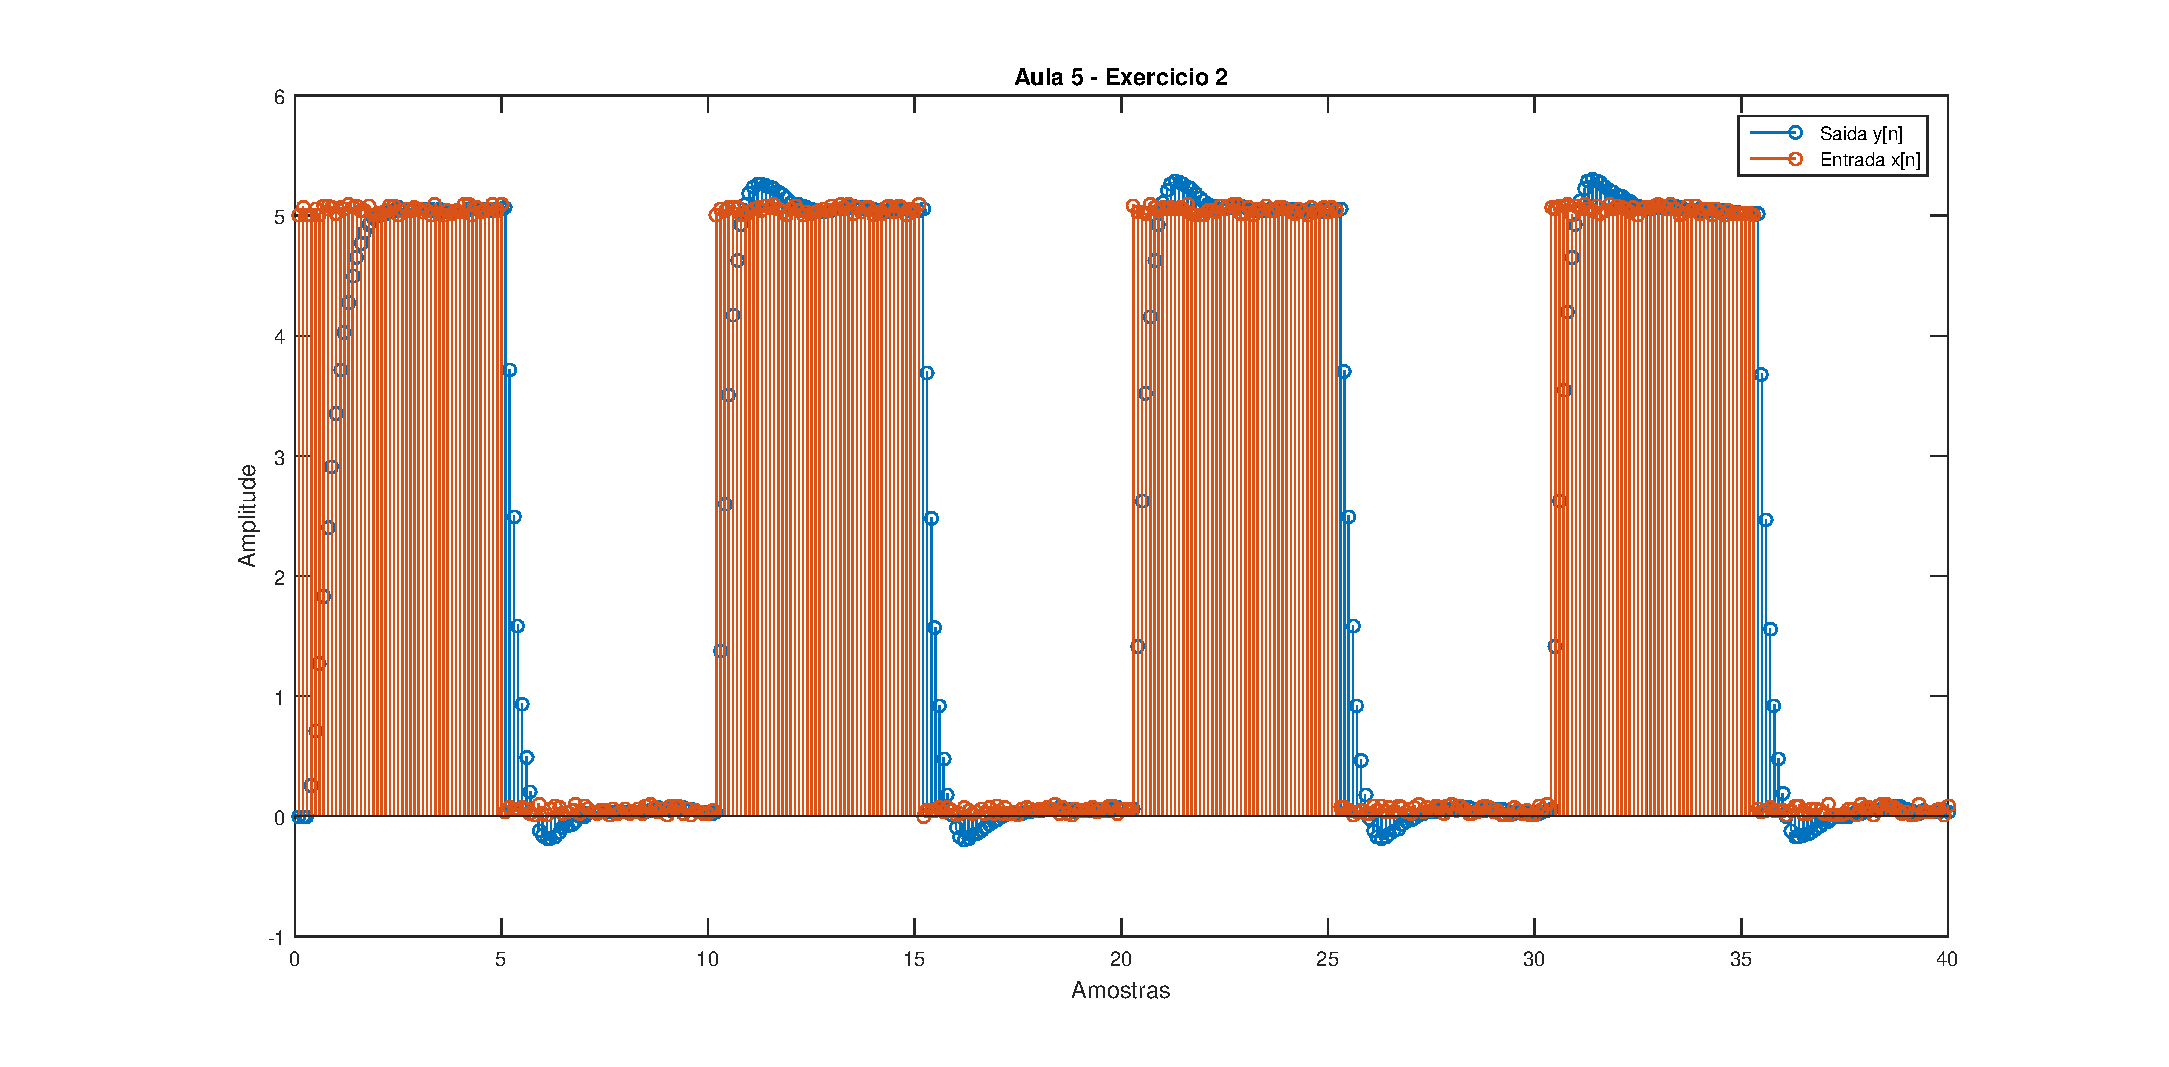
\includegraphics[scale = .66]{Imagens/Aula_5_exercicio2.eps}
      \caption{Gráfico de saída do código do exercício da prática 2.}
      \label{saida_ex2_pr_2}
  \end{figure}
\end{landscape}

\textcolor{red}{COMENTAR E DISCUTIR RESULTADOS}